\chapter{Geospatial Data on the Web}
\label{ch:ch1}

\begin{flushright}
\textit{``If you're a geospatial developer, AJAX is not a domestic cleaning product. \\
If you're a web dev, a polygon is not a dead parrot''}.\\
Steve Peters \\
(UK Government's Department \\for Communities and Local Government) 

\end{flushright}

%Content: raditional GIS data, soA on vocabularies, Contributions and conclusion \\
 
\section{Introduction}
%\todo{REUSE: this section below}
The increasing number of initiatives for sharing geographic information on the Web of data has significantly contribute to the interconnection of many data sets exposed as RDF based on the Linked Data principles. Many domains are represented in the Web of data (media, events, academic publications, libraries, cultural heritage, life science, government data, etc.) while DBpedia is the most used dataset for interconnection. For many datasets published, geospatial information is required for rendering data on a map. In the current state of the art, different approaches and vocabularies are used to represent the ``features'' and their geometric shape although the POINT is the most common representation making use of the latitude/longitude properties defined in the W3C Geo vocabulary. Other geometries from the OpenGIS standard (POLYGON, LINESTRING, etc.) are more rarely exploited (e.g. LinkedGeoData, GeoLinkedData) while fine-grained geometry representations are often required.

In France, the National Geographic Institute (IGN) has started to publish more and more data in RDF, as illustrated by the recent experimental LOD service \url{http://data.ign.fr}. IGN maintains large databases composed of different types of geographic entities, buildings, topographic information, occupied zones, etc. By reusing existing taxonomies and publishing them on the Web would ease the integration, retrieval and maintenance of French geospatial objects. Moreover, adding semantics to the current data on the Web will not only resolve ambiguities between datasets, but also will enable answering more complex queries than current GIS systems can handle, such as: ``\emph{show all buildings used as tribunal courts in the 7th Arrondissement of Paris}''. Another use-case is the possibility to reason over parts of a structure: ``\emph{show the points where the river Seine touches a boundary of a district in Paris that contain an activity zone}''.

In this Chapter, we first describe the notion of geographic information, with its specificity and diversity of formats (Section \ref{sec:geointro}). Then, we survey the models used on the Web to model existing geodata, by pointing some limitations (Section \ref{sec:vocgeoreview} and Section \ref{sec:currentmodel}. We then move to distinguish two levels of georeferencing data (direct and indirect), and the importance of CRSs in the interpretation of geodata (Section \ref{sec:georef}). The contributions start with a REST service for converting geodata in Section \ref{sec:rest-service}, followed by vocabularies developed both for handling geometries and features on the Web (Section \ref{sec:topovocab} and Section \ref{sec:geovocab}). The chapter closes with a take-away message



\section{Geographic Information}
\label{sec:geointro}
%\todo{Use some materials from Deliverable spatial data of Datalift- ADD part of the work of Nathalie thesis-
%ADD also Ruas thesis} \\

Geographical phenomena require two descriptors to represent the real world; \textit{what is represent,} and \textit{where it is.} as reported by authors in \cite{burrough98}. For the former, concepts such as ``town'', ``school'', ``river'', are used to recognize the phenomena and described in terms of well-established ``objects'' or `entities''. At the same time, the type of concepts used to describe a phenomena vary from one scale of resolution to another, depending on the perception of the human observation of the world. The space reference of the phenomena may be defined in terms of geometrically exact or a relative location. The former uses local or world coordinate systems -local or internationally accepted projections that uses geometrical coordinates of latitude and longitude - defined using a standard system of spheroids, projections, and coordinates \cite{burrough98}. Two approaches are generally used to represent geographical primitives in GIS: vector and raster approaches. In the vector data model, the space is represented by a geometry that describes the location and implicitly the shape, and information attributes such as the name, nature, length, or surface. In general, the geometry of a geographic object/entity can be described using three primitives:
\begin{itemize}
\item \textbf{Point} represented in terms of XY coordinates. For example. 
\item \textbf{Line} represented by a sets of XY coordinate pairs that define a connected path through space. 
\item \textbf{polygon} represented in terms of the XY coordinates of its boundary, or in terms of the set of XY coordinates that are enclosed by such as boundary. 
\end{itemize}    

Figure \ref{fig:vectormodel} shows for different representations of an address in the BD ADRESS\circledR \hspace{1pt} database, such as points, buildings, path, additional address location, etc.

\begin{figure}[ht!]
\centering{
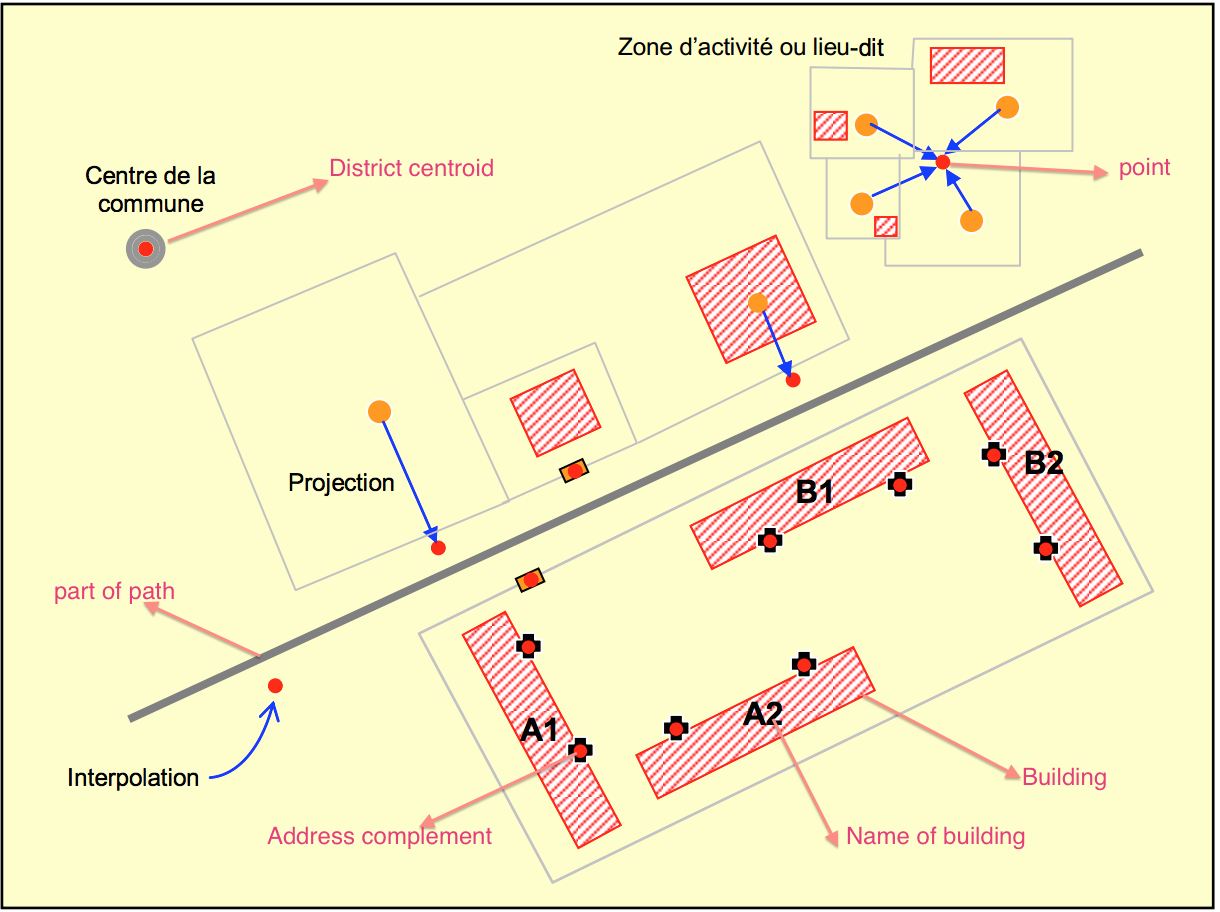
\includegraphics[scale=0.60]{img/vectorRepresentation.png}
\label{fig:vectormodel}
\caption{Vector representations of entities in  BD ADRESSE\circledR \hspace{1pt} produced by IGN-France.}
}
\end{figure}


\subsection{Specificity}
 Depending on the level of the spatial resolution, a phenomenon reveals more or less details, according to the intended use. So, increasing the level of resolution might reveals internal structure. For example, in the case of a town: sub-districts, suburbs, streets, houses, lamp-posts, traffic signs; which can be important for purpose and not for others. The level of details also influence the representation of a given entity, and thus provides different views of the same entity in a GIS. A town could be represented by a point at a continental level of resolution but as a polygon entity at a regional level. A road at national level is adequately represented by a line; at a street level it becomes an area of paving.
 
Moreover, geographical data are stored in different GIS according to two different resolution: the metric resolution and ``decametric'' resolution \cite{anamaria08}. Thus, making differences in volume of the data, the scale used to gather and view them, and most importantly their importance. Geodata providers explicitly provides details on the scales and the purpose of their datasets. Let's take the case of BDCARTO\circledR \hspace{1pt}, BDTOPO\circledR \hspace{1pt} and BD ADRESSE\circledR \hspace{1pt} of IGN-France (French mapping agency). BD CARTO\circledR \hspace{1pt} represents the elements using a decametric precision, and contains many themes: roads, administrative units, etc. It helps to manage data from 1 : 50 000 to 1 : 200 000 resolution.  BD TOPO is used for producing maps at 1: 25 000 scale, and represents the modelization in 3D of the territory and the amenities with addresses. BD ADRESSE is used for a precised location using the postal code in 1: 25 000 scale. 

The aforementioned constraints on abstraction, representation at different scales and requirements of geographical data create some issues both for users and producers. Those issues motivate the need for different relations between GIS datasets. The Web is a good medium to represent a real world phenomena with a unique Uniform Resource Identifier (URI) and associated semantic for referencing, interlinking and tracking the evolution over time. 
 

\subsection{Data Formats and Serialization}
Diverse formats are used to store and exchange geodata in traditional GIS. Some of them are proprietary or closed formats, other are standards defined by OGC. We list below some of the most used formats:
 
 \paragraph{ESRI Shapefile:}
 
 A shapefile stores non topological geometry and attribute information for the spatial
features in a data set. The geometry for a feature is stored as a shape comprising a set of
vector coordinates \cite{esri98}. Regarding this format, four files are processed: the three mandatory dBASE file (.dbf), index file (.shx) and main file (.shp), plus the metadata file (.prj) that describes the CRS used by the dataset. The schema and the type of the thematic and geometric attribute are extracted from the main and dBase file.

 \paragraph{Geospatial DBMS:}
 It is a Database that is optimized to store and query geospatial data, such as Oracle Spatial, PostGIS (a spatial extension to PostgreSQL), SpatialLite (a spatial extension to SQLite). 
 
 \paragraph{GML:}
 OGC standard encoding specification for geodata in XML that enables the storage, transport, processing and transformation of geographic information. GML serves as a modeling language for geographic systems as well as an open interchange format for geographic transactions on the Internet. As with most XML based grammars, there are two parts to the grammar: the schema that describes the document and the instance document that contains the actual data. A GML document is described using a GML Schema. GML is also an ISO standard (ISO 19136:2007) 
 
 \paragraph{Well-Known-Text (WKT):}
 Well-known text (WKT) is a text markup language for representing vector geometry objects on a map, spatial reference systems of spatial objects and transformations between spatial reference systems\footnote{\url{http://en.wikipedia.org/wiki/Well-known_text}}. The formats were originally defined by the Open Geospatial Consortium (OGC) and described in the specifications for geographic information -simple feature access- \cite{opengis2011}. 
 
 \paragraph{GeoJSON:}
 
GeoJSON is a format for encoding a variety of geographic data structures \cite{geojson}. A GeoJSON object may represent a geometry, a feature, or a collection of features. It also supports the following geometry types: Point, LineString, Polygon, MultiPoint, MultiLineString, MultiPolygon, and GeometryCollection. Features in GeoJSON contain a geometry object and additional properties, and a feature collection represents a list of features. GeoJSON is the data format of choice for developers which is widely implemented and supported by many tool chains.
The default (and strongly recommended) Coordinate Reference System is WGS84, but alternative systems can be specified. The recommended nomenclature for CRS systems is to use OGC (Open Geospatial Consortium) URNs, for example urn:ogc:def:crs:OGC::CRS84 (for WGS84). EPSG identifiers, originally from the European Petroleum Survey Group and now maintained by the International Association of Oil and Gas Producers (OGP) can also be used. Alternatively, the parameters for a CRS can be linked to by URL. 
The example below represents in GeoJSON the location (point) of ``Eurecom'':

\begin{verbatim}
{
  "type": "Feature",
  "geometry": {
    "type": "Point",
    "coordinates": [43.614151, 7.071414]
  },
  "properties": {
    "name": "EURECOM"
  }
}
\end{verbatim}

 
 \paragraph{KML:}
KML\footnote{\url{http://www.opengeospatial.org/standards/kml}} is a language for the visualization of geographic information in 2D (on a map) or 3D (on a globe), including annotation of maps and images. Hence it can be used to specify layers for use in creating maps in a GIS system.  A Placemark is one of the most commonly used features in Google Earth. It marks a position on the Earth's surface, using a yellow pushpin as the icon. The simplest Placemark includes only a \texttt{<Point>} element, which specifies the location of the Placemark.
A Placemark object contains the following elements:
\begin{itemize}
\item \textit{A name} that is used as the label for the Placemark
\item \textit{A description} that appears in the ``balloon'' attached to the Placemark
\item \textit{A Point} that specifies the position of the Placemark on the Earth's surface (longitude, latitude, and optional altitude)
\end{itemize}

KML can be used to carry GML content, and GML can be ``styled'' to KML for the purposes of presentation. KML instances may be transformed loosely to GML, however roughly 90\% of GML's structures (such as, metadata, coordinate reference systems, horizontal and vertical datums, etc.) cannot be transformed to KML\footnote{\url{http://en.wikipedia.org/wiki/Geography_Markup_Language}}. KML has very limited support for metadata as recommended by ISO 19115. The CRS in use is implicit and unique.

\section{Status of Vocabularies Usage for Geospatial Data}
\label{sec:vocgeoreview}

The publication \cite{demter-2012-ekaw} of statistics concerning the actual usage of vocabularies on the LOD cloud \footnote{\url{http://stats.lod2.eu}} provides not only an overview of best practice usage recommended by Tim Berners-Lee\footnote{\url{http://www.w3.org/DesignIssues/LinkedData.html}}, but also provides a rapid view of the vocabularies re-used in various datasets and domains. Concerning the geographic domain, the results show that W3C Geo\footnote{\url{http://www.w3.org/2003/01/geo/wgs84_pos}} is the most widely used vocabulary, followed by the \texttt{spatialrelations}\footnote{\url{http://data.ordnancesurvey.co.uk/ontology/spatialrelations}} ontology of Ordnance Survey (OS). At the same time, the analysis reveals that the property \texttt{geo:geometry} is used in $1,322,302,221$ triples, exceeded only by the properties \texttt{rdf:type} ($6,251,467,091$ triples) and \texttt{rdfs:label}\\($1,586,115,316$ triples). This shows the importance of geodata on the web. Table~\ref{tab:vocabLOD} summarizes the results for four vocabularies (WGS84, OS spatial relation, Geonames ontology and OS admin geography) where the number of datasets using these vocabularies and the actual number of triples are computed.

\begin{table*}[!htbp]
\centering{
\begin{tabular}{|l|c|r|c| }
\hline
\multicolumn{1}{|c|} {Ontologies} & \multicolumn{1}{c|}{\#Datasets} & \multicolumn{1}{c|}{\#Triples}& \multicolumn{1}{c|}{SPARQL endpoint}\\
\hline
W3C Geo  &   21 & 15 543 105 & LOD cache\\
OS spatialrelations &   10 & 9 412 167 & OS dataset\\
Geonames ontology &   5 & 8 272 905 & LOD cache\\
UK administrative-geography &   3 &  229 689 & OS dataset \\
\hline
\end{tabular}
\caption{Statistics on the usage of the four main geographic vocabularies (LOD cache should be understood as \texttt{http://lod.openlinksw.com/sparql/}). There are many more vocabularies used in the LOD cloud that contain also geographical information but that are never re-used.}
\label{tab:vocabLOD}
}
\end{table*}

\section{Current Modeling Approach}
\label{sec:currentmodel}
In this section, we review the different approaches used to model geographical data on the Web, with their advantages and limitations.

\subsection{Vocabularies for Features}
Modeling of features can be grouped into four categories depending on the structure of the data, the intended purpose of the data modeling, and the (re)-use of other resources.
\begin{itemize}
  \item (i): One way for structuring the features is to define high level codes (generally using a small finite set of codes) corresponding to specific
      types. Further, sub-types are attached to those codes in the classification. This approach is used in the Geonames ontology\footnote{\url{http://geonames.org/ontology/ontology_v3.0.rdf}} for codes and classes (A, H, L, P, R, S, T, U, V), with each of the letter corresponding to a precise category (e.g: A for administrative borders). Classes are then defined as \texttt{gn:featureClass a skos:ConceptScheme}, while codes are \texttt{gn:featureCode a skos:Concept}.
  \item (ii): A second approach consists in defining a complete standalone ontology that does not reuse other vocabularies. A top level class is used under which a taxonomy is formed using the \texttt{rdfs:subClassOf} property. The LinkedGeoData ontology\footnote{\url{http://linkedgeodata.org/ontology}} follows this approach, where the $1294$ classes are built around a nucleus of $16$ high-level concepts which are: \texttt{Aerialway, Aeroway, Amenity, Barrier, Boundary, Highway, Historic, Landuse, Leisure, ManMade},\\ \texttt{Natural, Place, Power, Route, Tourism, Waterway}. The same approach is used for the French GeOnto ontology (Section~\ref{sec:alignment}), which defined two high-level classes \texttt{ArtificialTopographyEntity} and \texttt{Natural\-TopographyEntity} with a total of $783$ classes.
  \item (iii): A third approach consists in defining several smaller ontologies, one for each sub-domain. An ontology network is built with a central ontology used to interconnect the different other ontologies. One obvious advantage of this approach is the modularity of the conceptualizing which should ease as much as possible the reuse of modular ontologies. Ordnance Survey (OS) follows this approach providing ontologies for administrative regions\footnote{\url{http://www.ordnancesurvey.co.uk/ontology/admingeo.owl}}, for statistics decomposition\footnote{\url{http://statistics.data.gov.uk/def/administrative-geography}} and for postal codes\footnote{\url{http://www.ordnancesurvey.co.uk/ontology/postcode.owl}}. The \texttt{owl:imports} statements are used in the core ontology. Similarly, GeoLinkedData makes use of three different ontologies covering different domains.
  \item (iv): A fourth approach consists in providing a \textit{nearly flat list} of features or points of interest. This is the approach followed by popular Web APIs such as Foursquare types of venue\footnote{\url{http://aboutfoursquare.com/foursquare-categories/}} or Google Place categories\footnote{\url{https://developers.google.com/maps/documentation/places/supported_types}}. For this last approach, we have built an associated OWL vocabulary composed of alignments with other vocabularies.
\end{itemize}


\subsection{Vocabularies for Geometry Shape}
The geometry of a point of interest is also modeled in different ways. We complete here the survey started by Salas and Harth~\cite{Salas2011}:
\begin{itemize}
  \item \textit{Point representation}: the classical way to represent a location by providing the latitude and longitude in a given coordinate reference system (the most used on the web is the WGS84 datum represented in RDF by the W3C Geo vocabulary). For example, Geonames defines the class \texttt{gn:Feature a skos:ConceptScheme} as a \texttt{SpatialThing} in the W3C Geo vocabulary.
  \item \textit{Rectangle} (``bounding box''): which represents a location with two points or four segments making a geo-referenced rectangle. In this way of modeling, the vocabulary provides more properties for each segment. The FAO Geopolitical ontology\footnote{\url{http://www.fao.org/countryprofiles/geoinfo/geopolitical/resource/}} uses this approach.
  \item \textit{List of Points}: the geometry shape is a region represented by a collection of points, each of them being described by a unique RDF node identified by a lat/lon value. The \texttt{Node} class is used to connect one point of interest with its geometry representation. The POI are modeled either as \texttt{Node} or as \texttt{Waynode} (surfaces). This approach is followed by LinkedGeoData~\cite{linkedgeodata}.
  \item \textit{Sequence of Points}: the geometry shape is represented by a group of RDF resources called a ``curve'' (similar to LineString of GML). The POI is connected to its geometry by the property \texttt{formedBy} and an attribute \texttt{order} to specify the position of each node in the sequence. This approach is the one used in GeoLinkedData~\cite{deLeon2010}.
  \item \textit{Literals}: the vocabulary uses a predicate to include the GML representation of the geometry object, which is embedded in RDF as a literal. This approach is followed by Ordance Survey~\cite{Goodwin2008}.
  \item \textit{Structured representation}: the geometry shape is represented as a typed resource. In particular, polygons and lines are represented with an RDF collection of basic W3C Geo points. This approach is used by the NeoGeo vocabulary\footnote{\url{http://geovocab.org/doc/neogeo/}}.
\end{itemize}

\subsection{GeoSPARQL Standard and specifications}
\label{sec:specgeosparql}

OGC-Simple Features Access standard aims to support both representing and querying geospatial data on the Semantic Web. The standard document~\cite{ogc2012} contains 30 requirements. It also defines a vocabulary for representing geospatial data in RDF and provides an extension to the SPARQL query language for processing geospatial data. 
Moreover, GEOSPARQL defines functions that request or check properties of a geometry (e.g., isSimple, isEmpty, Dimension, GeometryType, SRID), function that test test topological relations (e.g., contains),
and functions that construct new geometries from existing ones (e.g., buffer). 
 The proposed standard follows a modular design with five components: 
\begin{itemize}
\item (i) A \textit{core component} defining top-level RDFS/OWL classes for spatial objects; 
\item (ii) a \textit{geometry component} defining RDFS data types for serializing geometry data, RDFS/OWL classes for geometry object types, geometry-related RDF properties, and non-topological spatial query functions for geometry objects; 
\item (iii) a \textit{geometry topology component} defining topological query functions; 
\item (iv) a \textit{topological vocabulary component} defining RDF properties for asserting topological relations between spatial objects; and 
\item (v) a \textit{query rewrite component} defining rules for transforming a simple triple pattern that tests a topological relation between two features into an equivalent query involving concrete geometries and topological query functions.
\end{itemize}

 Each of the components described above has associated requirements. Concerning the vocabulary requirements, Table~\ref{tab:reqgeosparql} summarizes the seventeen requirements presented in the GeoSPARQL draft document.
\begin{table}
\centering{
\begin{tabularx}{\textwidth}{|X|X|l|}%{l|l|l}
\hline
Geo- 	& Requi-   & Implementation Definition \\ 
Aspect	& rement   &  \\ \hline
     	 		    & Req 2 		& The Class \texttt{SpatialObject} should be defined \& accepted\\
     	 		    & Req 3 		& Defines \texttt{Feature rdfs:subClassOf SpatialObject} \\
Feature			& Req 4 			& Defines $8$ Simple Features Object Properties(OP) \\
				& Req 5 			& Defines $8$ Egenhofer OP with domain and range \\
				& Req 6			  & Defines $8$ RCC OP with domain and range \\ \hline
				& Req 7 			& Defines \texttt{Geometry rdfs:subClassOf SpatialObject} \\
Geometry		& Req 8 			& Defines OP \texttt{hasGeometry} and \texttt{defaultGeometry} \\
				& Req 9 			& Defines $6$ Data Properties: e.g: \texttt{dimension, isEmpty, etc.}  \\ \hline
				& Req 10-13			& \texttt{wktLiteral} definitions \& URI encoding  \\
Seriali- 	& Req 14			& Defines \texttt{asWKT} to retrieve WKTLiteral  \\
	zation			& Req 15-17			& GMLLiteral should be accepted  \\
				& Req 18			& Defines \texttt{asGML} to retrieve GMLLiteral \\
\hline
\end{tabularx}
\caption{Requirements and implementations for vocabulary definitions in GeoSPARQL.}
\label{tab:reqgeosparql}
}
\end{table}


\subsection{Geospatial Vocabularies and Topological Functions}
\label{sec:topofunc}
%\todo{update the information in this section. link geosparql http://www.opengeospatial.org/standards/geosparql}

Based on the GeoSPARQL requirements, we were interested in comparing some geospatial vocabularies\footnote{\url{http://labs.mondeca.com/dataset/lov/vocabularySpace_Space.html}} to see how far they take already into account topological functions and which are the standard they followed among OpenGIS Simple Features (SF), Region Connection Calculus (RCC) and Egenhofer relations. We find that the NeoGeo (Spatial and Geometry) and OS Spatial vocabularies have integrated in their modeling partial or full aspects of topological functions as summarized in Table~\ref{tab:geosparql}.

As geodata has to be stored in triple stores with efficient geospatial indexing and querying capabilities, we also survey the current state of the art  in supporting simple or complex geometries and topological functions compatible with SPARQL 1.1. Table~\ref{tab:triplestore} shows which triple stores can support part of the GeoSPARQL standard regarding serialization and spatial functions.
\begin{table}
\begin{tabularx}{\textwidth}{|X|X|X|X|l}
\hline
\textbf{Geo-vocabulary} & \textbf{Topological Functions} & \textbf{GeoSPARQL Requirements} & \textbf{Standard Followed}\\
\hline
Ordnance Survey Spatial & \texttt{easting, northing, touches, within, contains} & Part of Req 4 & OpenGIS Simple Feature\\ \hline
Ordnance Survey Topography & \texttt{contains, isContainedIn} & Very small part of Req 4 & OpenGIS Simple Feature\\ \hline
Place Ontology & \texttt{in, overlaps, bounded\_by} & Small part of Req 4 & N/A\\
\hline
NeoGeo Spatial & All RCC8 relations & Part of Req 3; Req 6 & Region Connection Calculus (RCC)\\
\hline
NeoGeo Geometry & --- & Req 10 - 14 & N/A\\
\hline
FAO Geopolitical & \texttt{isInGroup, hasBorderWith} & -- & --\\
\hline
OntoMedia Space & \texttt{adjacent-below, adjacent-above, orbit-around, is\_boundary-of, has-boundary} & -- & --\\
\hline
\end{tabularx}
\caption{Comparison of some geo-vocabularies with respect to the GeoSPARQL requirements.}
\label{tab:geosparql}
\end{table}


\section{Georeferencing data on the Web}
\label{sec:georef}
Georeferencing data either by direct or indirect spatial reference requires some reference datasets that can be used as the spatial frame for anchoring these thematic data. Especially, it requires data on both CRSs and named places, which must be published on the Web of data.

\subsection{Identifying and describing CRSs on the Web}
In order to fulfill the need for CRS identification and description on the Web, OGC maintains a set of URIs for identifying the most commonly used CRS. While very useful, the main disadvantage of this proposal is that the URIs defined by OGC are not very intuitive for users who are not familiar with Spatial Reference System Identifiers defined by geographic information authorities like OGC or EPSG, such as ``4326'' (which actually refers to a WGS84 CRS defined by the EPSG). Moreover, many CRS commonly used locally, such as deprecated French projected CRS, are not available in that registry. In addition to OGC proposal, several registries have been proposed by the geographic information community for cataloguing existing CRSs.
The EPSG Geodetic Parameter Registry\footnote{\url{http://www.epsg-registry.org/}} allows querying the Geodetic Parameter Dataset gathered by the EPSG. CRSs can be retrieved by name, by code, by type or by coverage area, and their characteristics are displayed on a HTML form. Unfortunately, there is no direct access to these data through dereferenceable URIs.

\subsection{Direct georeferencing of data on the Web}
\label{sec:directgeo}
Modeling direct location information such as coordinates or vector data geometries in RDF still poses some challenges. In~\cite{Atemezing:TC12}, we have conducted a survey of the vocabularies used for representing geographical features from vocabularies of feature types to vocabularies for geometric primitives which provide ways for representing extents, shapes and boundaries of those features. 
Most of vocabularies dedicated to geometry representation reuse W3C Geo vocabulary which allows only WGS84 coordinates, such as NeoGeo\footnote{\url{http://geovocab.org/doc/neogeo/}}. With the rise of the Open Data movement, more and more publishers including governments and local authorities are releasing legacy data that are georeferenced using others CRSs. For example, IGN France releases data using different projected CRSs depending on the geographic extent of each dataset. In order to overcome this limitation on CRSs, the vocabulary designed by OGC GeoSPARQL standard  does not reuse W3C Geo vocabulary but proposes another class ``Point'' instead. Geometries of geographical data represented in RDF with the GeoSPARQL vocabulary are represented by literals encoded consistently with other OGC standards. \texttt{gsp:wktLiteral} and \texttt{gsp:gmlLiteral} are thus respectively derived from Well-Known Text and GML encoding rules. In \texttt{wktLiteral} and \texttt{gmlLiteral}, the CRS used to define the coordinates of the point is identified by a dereferenceable URI which is explicitly stated at the beginning of the literal. This way of associating coordinate reference systems with geometries has the advantage of being consistent with Linked Data principles: each CRS is identified with a dereferencable URI. The main drawback is that such literals cannot be easily queried with SPARQL, unless using regular expression-based filters.  To overcome this limitation, we propose in the geometry vocabulary presented in Section \ref{sec:geomvocab} to associate each geometry to the CRS used by its coordinates with the property \texttt{geom:crs}.

\subsection{Indirect georeferencing of data on the Web}
\label{sec:indirectgeo}

\subsubsection{Location Vocabulary}
The Location Core Vocabulary \footnote{\url{http://www.w3.org/ns/locn}} provides structure to describe a location in three different ways: by using a place name, a geometry or an address. The vocabulary is heavily based on the definition of IS0 19112 of a location, as "an identifiable geographic place." A part from using simple string labels or names, the vocabulary provides a property to allow a Location to be defined by a URI, such as GeoNames or DBpedia URI. The geographic name used for a spatial object is consistent with the INSPIRE Data Specification on Geographical Names \cite{inspire2009}. The Geometry Class denotes the notion of geometry at a conceptual level, and can be encoded in different formats including WKT, GML, KML, RDF+WKT/GML (GeoSPARQL), RDF (WGS84 lat/long, schema.org) and GeoHash URI references. In addition, 
the geometry property can be associated to either a literal (such as WKT, GML or KML) or a geometry class (e.g., ogc:Geometry and its subclasses, geo:Point, schema:GeoCoordinates and schema:GeoShape, a GeoHash URI reference). However, the CRS identifier of the geometry is either embedded in the literal (e.g., WKT, GML) or implicit in the more structured serialization (e.g., WGS84 lat/long), schema.org, GeoHash).

\subsubsection{Datasets using indirect georeferencing}
Modeling indirect location information such as administrative units or named points of interest in RDF is preferably done by identifying such geographic features with URIs and describing them by their properties, so that they can be referenced by other datasets. This is the case in one of the most reused datasets of the Web of data, namely Geonames\footnote{\url{http://sws.geonames.org/}}. However, there are yet very few reference datasets for the French territory on the Web of data.  A simple example is the current resource for \textit{Paris} in the French DBpedia\footnote{\url{http://fr.dbpedia.org/resource/Paris}}. The department's name associated to this resource is a literal named ``Paris'' and the different arrondissements composing the city are modeled as \texttt{skos:Concept} instead of \texttt{dbpedia-owl:Place}. Even Geonames data remain very limited, as French administrative units are provided as simple geometries (POINT). The ``Official Geographic Code''\footnote{\url{http://rdf.insee.fr/sparql}} published by the French Statistical Institute (INSEE) is the most up-to-date and accurate dataset on French administrative units, but unfortunately it contains no geometrical description of their boundaries. This has the consequence of not having a baseline during mapping process for application developers trying to consume specific data coming from France. Datasets describing administrative units, points of interest or postal addresses with their labels and geometries, and identifying these features with URIs could be used with benefits not only for georeferencing other datasets, but also for interlinking datasets georeferenced by direct and indirect location information.

%\todo{Discuss about locn and datasets published} \\
%\textcolor{red}{Describe the contributions on geometry and geography vocabularies. Reuse mainly the recent work to be presented at Terra Cognita 2014}


\section{A REST Service for Converting Geo Data}
\label{sec:rest-service}
%\todo{extend this section with current results of the implementations, comparison with existing tools}

\subsection{Datum}
The Earth is shaped like a flattened sphere. This shape is called an ellipsoid. A datum is a model of the earth that is used in mapping. The datum consists of a series of numbers that define the shape and size of the ellipsoid and it's orientation in space. A datum is chosen to give the best possible fit to the true shape of the Earth.
There are a large number of datum in use. Many of them are optimized for use in one particular part of the world. An example is the Geodetic 1949 datum that has been used in New Zealand. Another example, familiar to GPS users, is the WGS-84 datum. WGS-84 is an example of a datum that is used globally.
A point (location) is referenced by its longitude and latitude values. Longitude and latitude are angles measured from the earth's center to a point on the earth's surface. The angles often are measured in degrees (or in grads). It is important to keep in mind that latitude and longitude are always specified in terms of a datum. The latitude and longitude of one current position are different for different datums. For example, the \emph{``Th\'{e}\^{a}tre National de Nice''} in Nice, France is at \emph{43.700594\degree N, 7.277959\degree E} in WGS 84 coordinates and \emph{43.700570\degree N, 4.941204\degree E} in NTF coordinates, an old France CRS. If the latter coordinates are used in WGS 84, they will point to a position which is approximately \textit{295.17 kilometers} away from the theater. So when working with latitude/longitude coordinates and getting an error of a couple of hundred meters, it is most likely that the wrong datum is in used.

\subsection{Tools for converting Datum}
As we have seen, geodata interpretation relies on a coordinate reference system, and while the WGS84 CRS is the \textit{de-facto} standard for GPS devices, many other CRS are in used. For example LAMBERT 93, RGM 04 or RGR 92 are respectively used for georeferencing points of interests in France continental, Mayotte or La Reunion. We have developed a REST service that is capable of transforming one dataset using a particular CRS into another one. 

A software called Circ\'e\footnote{\url{http://geodesie.ign.fr/?p=53&page=circe}}, published by IGN, provides the abilities to convert coordinate between CRSs in France and WGS 84. It has two conversions mode: standard and grid. In both modes, the user is required to input the source CRS values in order to convert. Based on what datum and projection method used, the number of required fields are different. 
Circ\'e also has a batch converting mode which is done by supplying a file. The format of the content of the file is simple. The available formats are converted into \textsl{[location name] {Lat/Lon} {Lon/Lat} [Altitude/Height]}. There is an option to choose which format to use. But due to the fact that it is a closed source software, no one can use the software as a service for their system.

Another tool is a Web based application called the world coordinate converter at \url{http://twcc.free.fr}. This tool can convert between numerous of CRSs. Unlike Circ\'e which only supports France and WGS 84, this tool supports conversion of international CRSs and nationals' CRSs. The result output from these two tools are the same. However, just like Circ\'e, no API or any open service for the community to use their full power horse unless going to their website and use it like an application.

These tools are great as a standalone tool for end user, but not so great for developer community. The developer can only use them to test their result. There is no possible way to use their fully function algorithm unless develop it again. 
\paragraph{Our proposal:} The purpose of the REST Converter is to propose a web based service to perform conversion between various CRSs.

The algorithms implemented are the ones described at \url{http://geodesie.ign.fr/index.php?page=algorithmes} and available within the standalone Circ\'e software\footnote{\url{http://fr.wikipedia.org/wiki/Circe_(logiciel)}}.

At the moment, the following features are implemented in the Geo Converter:
\begin{itemize}
\item from/to WGS 84 to/from WGS 84 UTM ;
\item from/to WGS 84  to/from Lambert 93 and 
\item from/to WGS 84 UTM to/from Lambert 93
\end{itemize}   

The API can also convert a file with space separated values. The API supports JSON as one of the output format. The code of the REST service is available at \url{https://github.com/vienlam/Geo}.

\subsection{Algorithms Evaluation}

Figures Fig.\ref{fig:convertToLambert93} and Fig.\ref{fig:convertTowgs84utm} show the resulting conversion from our tool, Geo Converter, in comparison with Circ\'e and twcc.free.fr (TWCC).


\begin{figure}[!htbp]
\centering{
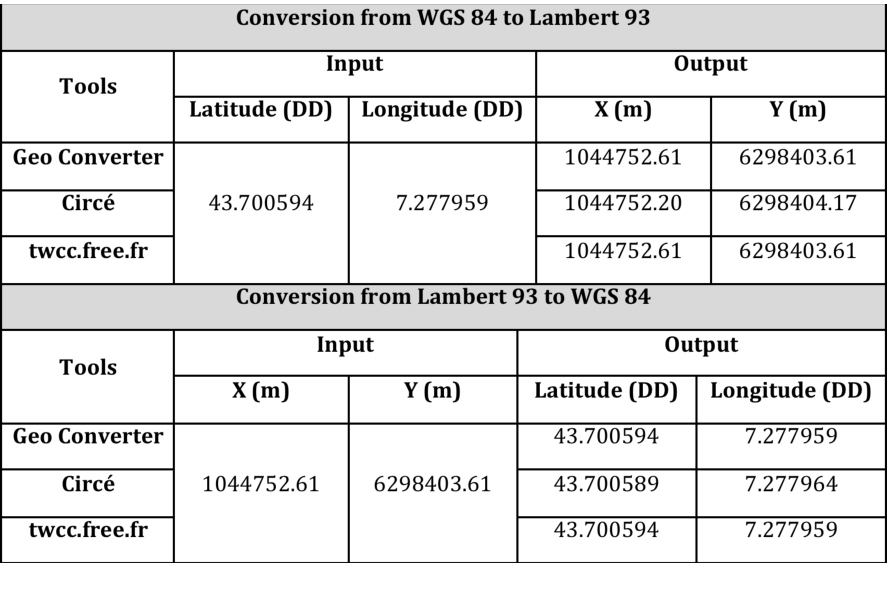
\includegraphics[scale=0.9]{img/conversion-wgs84-lambert93.pdf}
\caption{Results of conversion from WGS 84 to Lambert 93. Note: DD=Decimal Degree}
\label{fig:convertToLambert93}
 }
\end{figure}


\begin{figure}[!htbp]
\centering{
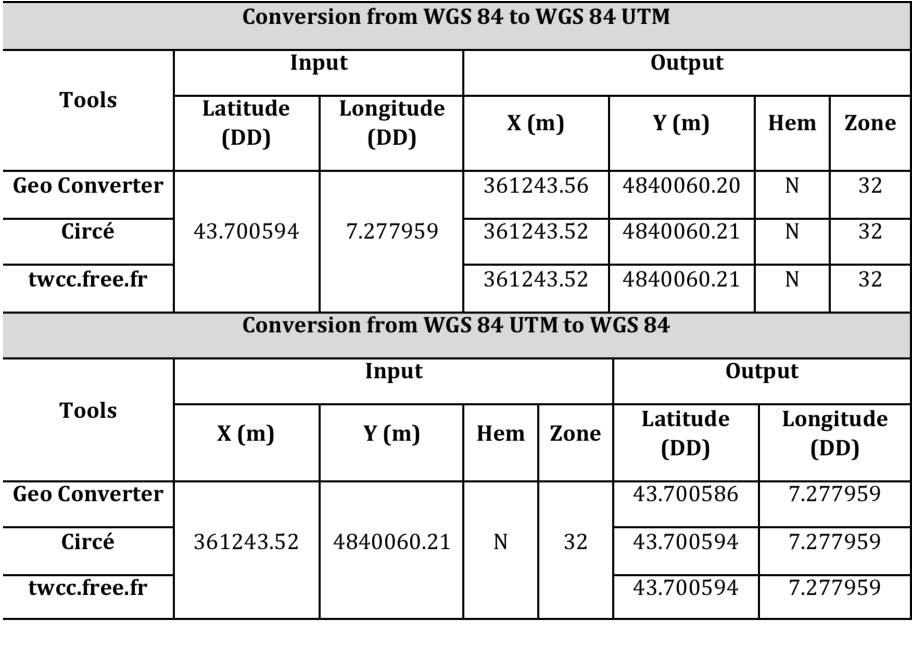
\includegraphics[scale=0.9]{img/conversion-wgs84-wgs84utm.pdf}
\caption{Results of conversion from WGS 84 to WGS 84 UTM. DD=Decimal Degree }
\label{fig:convertTowgs84utm}
 }
\end{figure}

 The results show that the results from Geo Converter are not too much different from Circ\'e and TWCC. This deviation can be tolerated, since when showing on the map, they are basically the same point.
There is no need for evaluation of conversion between Lambert 93 to UTM, since it is needed an intermediate step of convert to WGS 84. The conversion from Lambert 93 to WGS 84 works well, as well as from WGS 84 to WGS UTM. 


\subsection{API Access and Parameters}
\label{sec:access}

\subsubsection{Simple Converter}
The API is working through URL like any RESTful service does. The syntax for the service is (note that \{\} is required and [] is optional):
\url{http://{domainname}/eurecom.geo.rest/api/converter/{D1}[P1]{D2}[P2]?{Parameters}} \\
Where: \\
\texttt{domainname}: Eurecom domain name.\\
\texttt{D1} and \texttt{D2}: Datum of source and target CRS respectively.\\
\texttt{P1} and \texttt{P2}: Projection of source and target CRS respectively.\\
\texttt{Parameters:} The required parameters as input to the service. See table below for detail of required parameters for each converter. Parameters are provided as p1=v1\&p2=v1 where p1 is the first parameter with v1 is its value, etc.\\
An example can be:
\begin{verbatim}
eurecom.fr/eurecom.geo.rest/api/converter/WGS84RGF93Lambert93?lon=4.7021484375&
lat=45.2130035559939
\end{verbatim}

\subsubsection{Batch Converter}
The API also support batch converter by using file. The URL syntax is:
\begin{verbatim}
http://{domainname}/eurecom.geo.rest/api/converter/file/
{D1}[P1]{D2}[P2]?{Parameters}
\end{verbatim}

Where D1, P1, D2, and P2 is as before. The parameters are the source file, and the encoding system. 
The order of the input coordinates in the file is matter, so the exact order is as follow:
{longitude/x} {latitude/y} [zone] [hemisphere]
The first value should be longitude, in case geographic coordinate, or x, in case of planimetric coordinate. The second value is latitude or y. In case of UTM coordinates, the following third value is the zone. The last value is hemisphere. 

\subsubsection{Result Format}
Normally, the API will return the result in form of normal string with the space character as delimiter for each coordinate. In case of batch converter, each location will be in one line. For example:
\begin{verbatim}
eurecom.fr/eurecom.geo.rest/api/converter/WGS84RGF93Lambert93?lon=4.7021484375&
lat=45.2130035559939
\end{verbatim}

will return a string of:
\begin{verbatim}
833607.9336802219 6458515.660215093
\end{verbatim}

The order of value respond to the order of coordinate as follow:
\begin{verbatim}
{longitude/x} {latitude/y} [zone] [hemisphere]
\end{verbatim}

\paragraph{JSON format result:}
However, one can ask the API to return the result string in JSON format. To demand the API to do so, simply put the json parameter with the value 1 to the link. For example:
\begin{verbatim}
eurecom.fr/eurecom.geo.rest/api/converter/WGS84RGF93Lambert93?lon=4.7021484375&
lat=45.2130035559939&json=1
\end{verbatim}

will return a string in JSON format (no line breaking):
\begin{verbatim}
{"y":6458515.660215093,"x":833607.9336802219}
\end{verbatim}

JSON format return can also be applied for batch converter. The command is as before. An example of JSON format return of batch converter from WGS84 to Lambert93:

\lstset{basicstyle=\scriptsize, backgroundcolor=\color{white}, frame=single, caption= {Sample output of the batch converter}, label=snapshot, captionpos=b}
\begin{lstlisting}
{"point1":{"y":6543019.59988031,"x":882408.2999938729},"point2":{"y":6544401.599880268,"x":881947.5999938913},"point3":{"y":6581538.799879094,"x":849722.3999950405},"point4":{"y":6561282.999879616,"x":917481.0999927416},"point5":{"y":6561139.999879618,"x":917474.5999927415}}
\end{lstlisting}

For better human readable result, a tool such as JSONLint\footnote{ \url{http://jsonlint.com/}} can be used for the JSON format.


\subsection{User Interface}
To access the User Interface (UI), the URL is: \url{http://{domainname}/eurecom.geo.rest/}. Figure \ref{fig:uiconverter} shows the landing page of the converter. The UI shows two systems, which are the source and the target system, to provide input. Which system is source or target depend on which button at the end is used. If the button \textit{Convert S1-S2} is clicked, then the System 1 will be the source and System 2 is the target, and \textit{vice versa} for button \textit{Convert S2-S1}.
The required inputs is just as mentioned before. First is the datum to use. Next is the projection method. If no project method is used then choose None. Next is the inputs of the source system.
The map under the form will show where the coordinate in the source system point to through a marker. This marker can be used as an input to the source system as well.
By dragging the marker, the system will update the input values of the source system, which is the system that have the last edited field or act as source system in last conversion, to correspond to the marker position. Furthermore, the "Use Marker's Position" button can be used to take marker's position and convert it to the system which the button resides in. This will not change the source system.


\begin{figure}[!htp]
\centering{
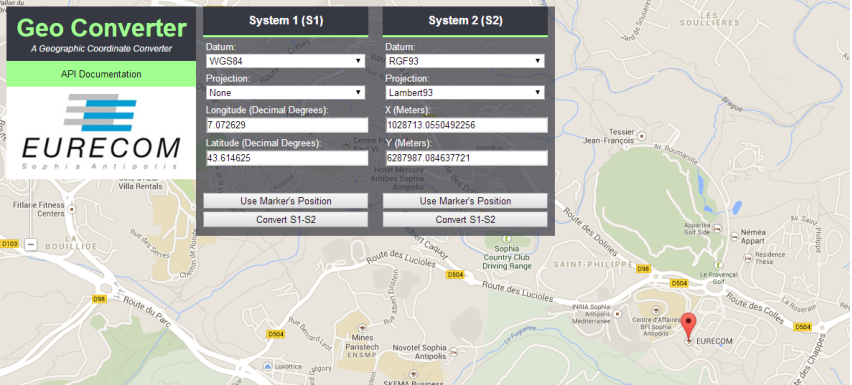
\includegraphics[scale=0.9]{img/UIconverter.pdf}
\caption{The User Interface of the Geo Converter}
\label{fig:uiconverter}
 }
\end{figure}


\section{Best Practices for Modeling Geospatial vocabularies}
\label{sec:bpgeo}

In~\cite{Atemezing:TC12}, we already surveyed numerous vocabularies for representing geographical features and their geometries, either using a literal (e.g. wktLiteral) or a structured representation \`a la NeoGeo. We concluded the survey with some recommendations for geometry descriptions:
\begin{itemize}
 \item the distinction of geometry versus feature and a property linking both classes (e.g. for attaching provenance information on how some points of a geometry have been collected),
 \item the ability to represent structured geometries (e.g. for performing simple spatial queries on the data, even when they are stored in a triple store that do not implement the GeoSPARQL standard),
 \item the integration of any coordinate reference system  (e.g. for allowing projected coordinates for cartographic purposes).
\end{itemize}
In addition to these recommendations, we also think that the domain of the property used to link a feature to its geometry should be left empty in order to accept links between any type of resource and a geometry. This would be useful for example, to associate a person to the coordinates of their birthplace.

\subsection{Some Recommendations}
The alignment of existing taxonomies for describing geodata enables interoperability of symbolic descriptions. The need for a better choice of geometric structure, typically the choice between literal versus structured representations depends on three criteria: 
\begin{itemize}
\item (i) the coverage of all the complex geometries as they appear in the data;
\item (ii) a rapid mechanism for connecting ``features'' to their respective ``geometry'';
\item (iii) the possibility to serialize geodata into traditional formats used in GIS applications (GML, KML, etc.) and
\item (iv) the choice of triple stores supporting as many as possible functions to perform quantitative reasoning on geodata.
\end{itemize}
    
    It is clear that a trade-off should be made depending on the technological infrastructure (e.g: data storage capacity, further reasoning on specific points on a complex geometry). The following points helps understanding better some of the challenges: 

\begin{itemize}
\item\textbf{Complex Geometry Coverage:} We have seen that on the Web of Data, there are few modeling of geodata with their correct shape represented as a LINE or POLYGON. However, some content providers (e.g. IGN) need to publish all types of geodata including complex geometries representing roads, rivers, administrative regions, etc. Two representations are suitable: \textit{OS Spatial} and \textit{NeoGeo} ontologies (Table~\ref{tab:reqgeosparql}). Direct representation of the GeoSPARQL vocabulary is also suitable.
\item \textbf{Features connected to Geometry:} In modeling geodata, we advocate a clear separation between the features and their geometry. This is consistent with the consensus obtained from the different GeoVocamps\footnote{\url{http://www.vocamp.org}} and the outcome of this approach is expressed in the modeling design of NeoGeo. The top level classes \texttt{spatial:Feature} and \texttt{geom:Geometry}are connected with the property \texttt{geom:geometry}.

\item \textbf{Literal versus structured Geometry:} Decomposing a LINE or a POLYGON into multiple results in an ``explosion'' in the size of the dataset and the creation of numerous blank nodes. However, sharing points between descriptions is a use case with such a need. IGN has such use-cases and the natural solution at this stage is to consider reusing the NeoGeo ontology . The choice of the triple store (e.g.,Virtuoso vs Open Sahara) is not really an issue, as the IndexingSail\footnote{\url{https://dev.opensahara.com/projects/useekm/wiki/IndexingSail}} service could also be wrapped on-top of Virtuoso to support full OpenGIS Simple Features functions\footnote{\url{http://www.opengeospatial.org/standards/sfs}}.
\end{itemize}


\section{Vocabularies for Geometries and Feature Types} \label{sec:topovocab}

Direct georeferencing of data implies representing coordinates or geometries and associating them to a CRS.  This requires vocabularies for geometries and CRSs. Besides, indirect georeferencing of data implies associating them to other data on named places. Preferably, these data on named places should be also georeferenced by coordinates in order to serve as basis for data linking between indirectly and directly georeferenced datasets. In this section, we present the vocabularies that we have defined and reused for geographic data publishing.
This requires reference geographic data on named places and therefore vocabularies for describing feature types and their properties. 

\subsubsection{A vocabulary for geometries} \label{sec:geomvocab}

On the current usage of georeferencing resources on the Web of data, it is assumed that the coordinates should be in WGS84, and hence the definition of the point. However, publishers might have data in different CRSs according to the location. Thus, our proposal is to define a more generic class for a POINT  with the benefit of choosing the CRS of the underlying data, as depicted in the Listing 2.3. 
The naming convention used for the \texttt{geom} vocabulary follows the terms used by the Simple Features vocabulary. The French translation of terms is based on the glossary of multilingual terminology of ISO/TC 211 available at \url{http://www.isotc211.org/Terminology.htm}.

\begin{deflda}:
A resource of type \texttt{geom:Geometry} should be associated to exactly one resource of type \texttt{ignf:CRS} via the property \texttt{geom:crs}.
\end{deflda}

\begin{deflda}:
\textbf{A POINT} is a subclass of a \textbf{GEOMETRY}.
\end{deflda}

Regarding alignments with some existing vocabularies, the class \texttt{geom:Geometry} is a subclass of both \texttt{sf:Geometry} and \texttt{ngeo:Geometry}. The class contains in addition the property \texttt{geom:crs}. Moreover, it is possible to obtain equivalences between data modeled with \emph{ngeo} vocabulary and \emph{geom} vocabulary. The following SPARQL query make it possible:

\lstset{basicstyle=\scriptsize, backgroundcolor=\color{white}, frame=single, caption= {SPAQRL Query for creating sameAs links between data modeled with \emph{ngeo} and \emph{geom} vocabularies }, label=sameAsquery, captionpos=b}
\begin{lstlisting}

CONSTRUCT {
   [] a geom:Point;
    	owl:sameAs  ngeo:Point.
 
} WHERE {
 [] a geom:Geometry;
	geom:Point;
	geom:systCoord
<http://data.ign.fr/id/ignf/crs/WGS84G>.
}

\end{lstlisting}


\begin{deflda}:
An instance of the class \texttt{geom:Point} is associated with exactly one instance of \texttt{ignf:CRS} via the property \texttt{geom:crs}. An instance of a \texttt{geom:Point} has exactly one coordinate X and exactly one coordinate Y. The coordinates are \texttt{xsd:double} and referred to the following properties:
\begin{itemize}
 \item \texttt{geom:coordX} refers to, in an ellipsoidal CRS, the longitude of a point and within a projected CRS, the value of false easting of a point.
 \item \texttt{geom:coordY} refers to, in an ellipsoidal CRS, the latitude of a point and within a projected CRS, the value of false northing of a point.
\end{itemize}
\end{deflda}


\lstset{basicstyle=\scriptsize, backgroundcolor=\color{white}, frame=single, caption= {Definition in Turtle of the axiom defining a POINT. }, label=point, captionpos=b}
\begin{lstlisting}
geom:Point a owl:Class;
  rdfs:label "Point"@en, "Point"@fr;
  rdfs:subClassOf geom:Geometry;
  owl:equivalentClass
    [a owl:Class ;
	  owl:intersectionOf
		([a owl:Restriction;
		   owl:onDataRange xsd:double;
		   owl:onProperty geom:coordY;
	       owl:qualifiedCardinality "1"^^xsd:nonNegativeInteger]
         [a owl:Restriction;
		   owl:onDataRange xsd:double;
		   owl:onProperty geom:coordX;
		   owl:qualifiedCardinality "1"^^xsd:nonNegativeInteger])
     ] ;
     rdfs:subClassOf sf:Point.
\end{lstlisting}

\begin{deflda}
(PointsList): A \texttt{geom:PointsList} is a subclass of rdf:List. An instance of \texttt{geom:PointsList} is composed of only instances of type \texttt{geom:Point}.

\end{deflda}

\subsubsection{Extending GeoSPARQL vocabulary}
In order to fulfill these recommendations, we have developed a new vocabulary that re-uses and extends the existing vocabularies for representing geometries, namely:
\begin{itemize}
 \item \url{http://www.opengis.net/ont/geosparql#} (prefix \texttt{gsp}). This vocabulary provides the basic concepts to represent geographical data such as SpatialObject, Feature or \texttt{Geometry}. A Feature is linked to a Geometry via the relation \texttt{gsp:hasGeometry}. The geometries are typed strings (\texttt{gsp:gmlLiteral} or \texttt{gsp:wktLiteral} corresponding respectively to the properties \texttt{gsp:asGML} and \texttt{gsp:asWKT}). The vocabulary contains also spatial functions.
 \item \url{http://www.opengis.net/ont/sf#} (prefix \texttt{sf}): This vocabulary is based on the OGC standard Simple Features Access \cite{iso2004}. The class \texttt{sf:Geometry} is a subclass of \texttt{gsp:Geometry}. 
\end{itemize}
 
Reusing and extending GeoSPARQL Simple Features vocabulary with structured geometries  \`a la NeoGeo enables us to represent geometries both with GeoSPARQL compliant literals and with structured geometries that can be handled easily with SPARQL. The extension for structured geometries consists in defining a subclass for each class from the \texttt{sf} vocabulary, and defining properties to associate its instances with a CRS and coordinates or other suitable geometric primitives. For example, the class \texttt{geom:Point} is a subclass of \texttt{sf:Point}. An instance of \texttt{geom:Point} is associated with exactly one instance of \texttt{ignf:CRS} via the property \texttt{geom:crs}, and it
has exactly one coordinate X and exactly one coordinate Y. It can also have a Z coordinate. The coordinates are \texttt{xsd:double} and correspond to the properties \texttt{geom:coordX:}, \texttt{geom:coordY:} and \texttt{geom:coordZ:} respectively. Other complex geometries are also defined, such as Linestrings, LinearRings, Polygons or MultiPolygons. Their definitions are based on the class \texttt{geom:Point}. As an example, an instance of \texttt{geom:Linestring} is defined as an instance of \texttt{geom:PointsList} which is an ordered \texttt{rdf:List} of instances of \texttt{geom:Point} designated by the property \texttt{geom:points}.


We have also defined a property \texttt{geom:geometry} with an empty domain. Thus, our proposal defines a more generic class for a \textsf{POINT} with the benefit of choosing the CRS of the underlying data. Figure \ref{fig:geomcrs} gives an overview of the relationships between the high level concepts with geometries, CRS and topographic features.

\begin{figure}[!htbp]
\vspace{-13pt}
  \begin{center}
  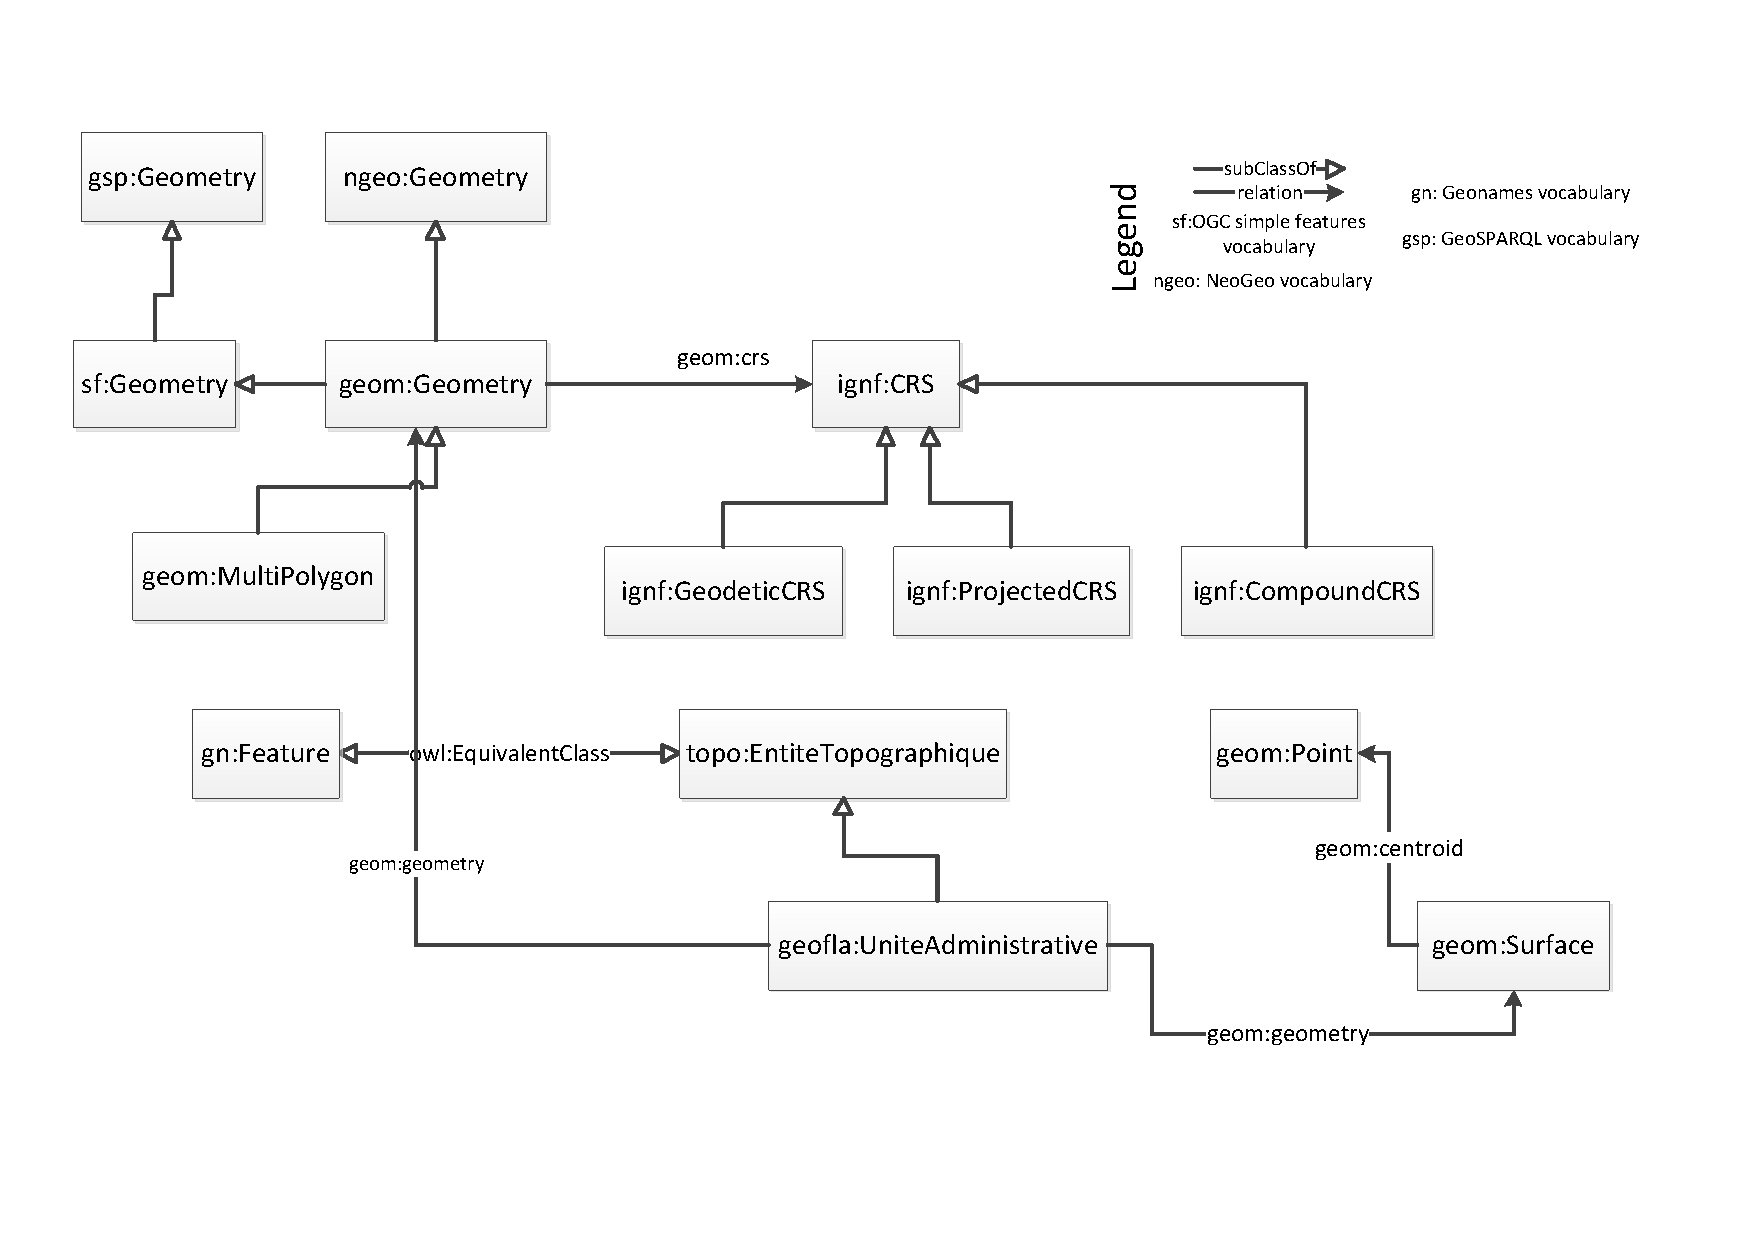
\includegraphics[width=0.9\textwidth]{img/vocabs-ign.pdf}
  \vspace{-15pt}
  \caption{High level classes of ignf, geom and topo vocabularies; relationships between them and mappings with external vocabularies.}
  \vspace{-10pt}
  \label{fig:geomcrs}
  \end{center}
\end{figure}

\subsection{A vocabulary for Topographic entities}
\label{sec:topovocab}

A topographic entity \texttt{topo:EntiteTopographique} is the class associated to a phenomenon with an associated location on the Earth\footnote{The names used in the description of the classes or properties are rdfs:label[@lang='en'] of the actual URIs in the models.}. \texttt{topo}\footnote{\url{http://data.ign.fr/def/topo}} vocabulary contains $8$ direct subclasses: Buildings and structures, Cableway transport line, Energy transport infrastructure, Inland hydrographic feature, Relief feature, Road transport feature, Transport by rail feature, Vegetation area and Working area of interest. Furthermore, we use a second level of classes to model direct subclasses of the previous ones. For example, a Building is specialized in $6$ different classes: Cemetery, Sports ground, Structure, Tank and Taxiway. A building is then connected with the property \texttt{topo:typeDeBatiment} (type of building) to different \textit{`nature'} of buildings, which are modeled as SKOS concepts. SKOS is intensively used to easily group concepts into different schemes (using \texttt{skos:hasTopConcept}) and provide semantic relationships (e.g: \texttt{skos:broader}, \texttt{skos:narrowMatch}) among them. This gives flexibility in the model by defining few high level classes and restrictions for the properties. Table ~\ref{tab:skosConcepts} gives a listing of the different SKOS namespaces defined to capture some high level concepts.

\begin{table}[!htb]
\centering{
\begin{tabular}{ll}
\specialrule{1pt}{1pt}{1pt}
 \textbf{URL}	 & \textbf{Description} \\ \specialrule{1pt}{1pt}{1pt}
  cdtopo:typedezai:liste &  list of different areas of activities and interest\\ 
  cdtopo:typedebatiment:liste & list of types of buildings \\
  cdtopo:typedeterraindesport:liste & list of types of sports ground \\
  cdtopo:typedeconstruction:liste & list of types of construction \\
  cdtopo:typedereservoir:liste & list of types of tanks \\
  cdtopo:typedevegetation:liste & list of types of vegetation \\
  cdtopo:typederelief:liste & list of types of relief \\
  cdtopo:typedevoieferree:liste & list of types of railway track \\
  cdtopo:typedetransportcable:liste & list of types of cableway transport \\
  cdtopo:typedefranchissement:liste & list of types of crossing \\
  cdtopo:typederoute:liste & list of types of road \\
  cdtopo:typedereservoir:liste & list of types of waterhole \\
  cdtopo:typedelaisse:liste & list of types of tide line \\
  
		\\ \specialrule{1pt}{1pt}{1pt}

\end{tabular}
\caption{List of concept schemes used in the topographic ontology.  }
\label{tab:skosConcepts}
}
\end{table}

\subsection{Publishing structured geometries from geographic data}
The vocabulary for geometry reused by a geodata converter that takes traditional GIS data as input and outputs RDF data with geometries defined both with a \texttt{gsp:wktLiteral} and with a structured representation compliant with our vocabulary. Geometries are automatically associated with the chosen CRS. This converter is implemented as a plugin of the Datalift platform (cf. Section \ref{sec:geomRDF}) and can be reused easily for geographic data publishing purpose.


\subsection{CRS requirements for the  French territory} \label{sec:reqs}

As explained in Section \ref{sec:context}, making explicit the CRS used in a given dataset is a very important issue when dealing with direct location data. This is especially important in the field of geographical information where different CRSs are commonly used due to technical or legal requirements. For INSPIRE Directive, CRS are considered as reference data used for linking thematic data \cite{inspire2009}, and must be described according to ISO 19111 standard. To be consistent with Linked Data principles, CRS should be identified by URIs, like in OGC proposal. Moreover, as Linked Data users are not always familiar with CRS identifiers commonly used within the geographic information community, URI used to identify CRS should use more intuitive names. Finally, consistently with our goal of contributing to a better georeferencing of data on the French territory, we need an access to the descriptions of all French CRSs, including some deprecated but still used CRSs like ``Lambert 1''.

\begin{table}[!htp]
\centering{
\begin{tabular}{lr}
\specialrule{1pt}{1pt}{1pt}
 \textbf{Prefix}	& 	\textbf{URI}	  \\ \specialrule{1pt}{1pt}{1pt}
geofla 	   & \url{http://data.ign.fr/def/geofla#}  \\
geom &  \url{http://data.ign.fr/def/geometrie#} \\
ignf &  \url{http://data.ign.fr/def/ignf#} \\
rgeofla &  \url{http://data.ign.fr/id/geofla/} \\
topo &  \url{http://data.ign.fr/def/topo#} \\
rtopo &  \url{http://data.ign.fr/id/topo/} 

		\\ \specialrule{1pt}{1pt}{1pt}
\end{tabular}
\caption{ URI schemes and conventions used for vocabularies and resources.}
\label{tab:uris}
}
\end{table}

The Information and Service System for European Coordinate Reference Systems\footnote{\url{http://www.crs-geo.eu}}  provides an access to ISO 19111 standard-based descriptions of the main European CRSs but has the same limitation as the EPSG registry: access to the descriptions is not allowed by URI, but only through a cartographic interface.
\url{SpatialReference.org} initiative aims at allowing users to use URI-based references to spatial reference systems, including some CRSs defined and maintained by IGN France.  Besides, the proposed URL policy is not very intuitive. As an example, this URL identifies the projected system defined by IGN France, Lambert 93: \url{http://spatialreference.org/ref/sr-org/7527/}. Moreover, the definitions of some deprecated CRSs such as Lambert zone projected CRSs (which are still used in some datasets) seem to be referenced only for the authority EPSG and not for IGNF, which also maintains a registry of CRSs. ISO 19111 standard-based definitions of all CRSs defined and maintained by IGN France are  published in an XML file\footnote{\url{ http://librairies.ign.fr/geoportail/resources/IGNF.xml}}.
References to equivalent definitions provided by the EPSG registry are explicitly stated with EPSG SRID. CRSs are identified by URIs using short names instead of numeric codes. For example, \url{http://registre.ign.fr/ign/IGNF/crs/NTFLAMB2E}  is the URI designed for the ``Lambert 2 \'{e}tendu'' projected system. Indeed ``NTFLAMB2E'' is used to identify the projected system ``Lambert 2 \'{e}tendu'' which is based on NTF (New French Triangulation) geodetic reference system. Unfortunately, this registry is still in evolution and its URIs are not dereferenceable yet.

\begin{figure}[!htbp]
 \begin{center}
  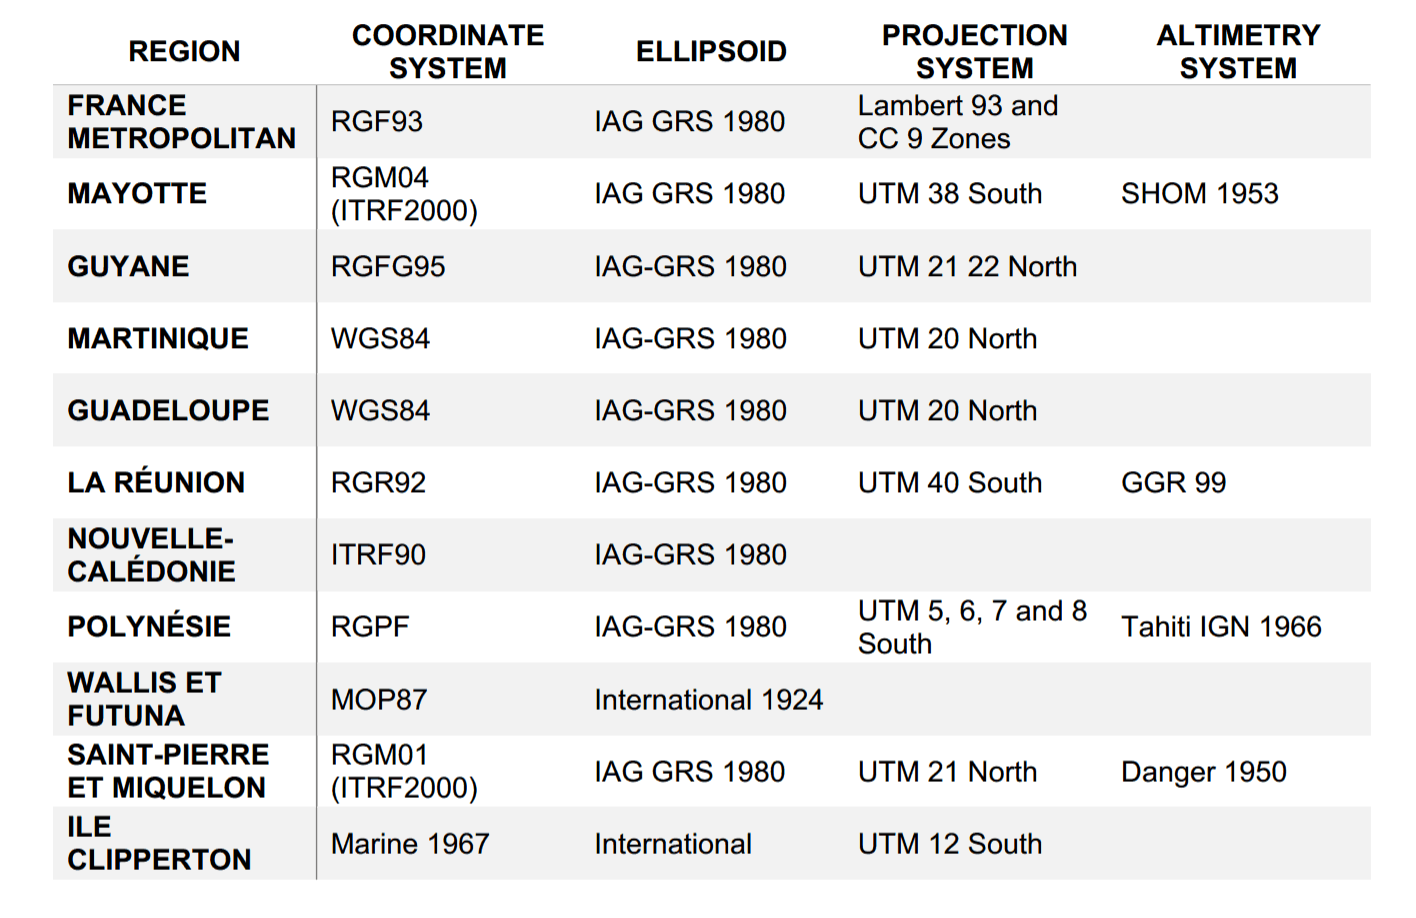
\includegraphics[width=120mm]{img/crs-france.png}
  \caption{Coordinate Reference Systems used in France}%\footnote{Source: \texttt{http://geodesie.ign.fr/}}
  \label{fig:crsinfr}
 \end{center}
\end{figure}
 
%\paragraph{Publishing a dataset on French CRSs}
As no existing registry fulfilled all our requirements, we have developed a vocabulary\footnote{\url{http://data.ign.fr/def/ignf}}, inspired from the ISO 19111 schema for CRSs description. Then we have converted IGNF CRSs registry into RDF, and published this dataset on the Web with the Datalift platform\footnote{A service to lookup CRS in RDF can be found at \url{http://www.eurecom.fr/~atemezin/ignf-lookup/}}. Therefore, the description of the ``NTF Lambert 2 \'{e}tendu'' projected CRS can be retrieved at this URL \url{http://data.ign.fr/id/ignf/crs/NTFLAMB2E}.

\section{Vocabularies for Geographic Feature Types}
\label{sec:geovocab}

Indirect georeferencing of resources on the Web requires reference geographic data on named places and therefore vocabularies for describing feature types and their properties. Therefore, we have chosen to publish a reference dataset on administrative units called GEOFLA\circledR, which is already available in GIS format under an Open Data license. We have also made tests of data conversion and interlinking with another largest dataset on French names places. We have produced and published two vocabularies to describe these datasets, to make sure that all concepts and properties needed would be available.
In the GEOFLA\circledR ~vocabulary, 5 classes have been defined: commune, canton, arrondissement, department and region. In the BD TOPO\circledR ~vocabulary\footnote{\url{http://data.ign.fr/def/topo}} \emph{}$35$ main classes have been defined. They represent the main types of geographic features represented in the BD TOPO\circledR ~database. In both vocabularies, properties have been defined based on the attributes of their related classes in the databases. The geographic feature types defined as values of attributes ``nature'' are modeled as instances of \texttt{skos:Concept}. SKOS is intensively used to easily group concepts into different schemes (using \texttt{skos:hasTopConcept}) and provide semantic relationships (e.g: \texttt{skos:broader}, \texttt{skos:narrowMatch}) among them. We also provide alignments with Geonames vocabulary, where \texttt{topo:Place} is subclass of \texttt{gn:S} and \texttt{owl:sameAs} linked concepts.\footnote{\url{https://github.com/gatemezing/ign-iswc2014/blob/master/vocabularies/mappingsGeonames.ttl}} 

All the classes are defined as subclasses of  \texttt{topo:EntiteTopographique} which defines the representation of a real world entity associated to a location relative to the Earth, consistently with ISO TC 211 and OGC standards. 
The GEOFLA\circledR 's application schema is composed of classes representing different types of french administrative units, namely communes, cantons, arrondissements and departments. In \texttt{geofla} vocabulary, we add a class \texttt{Region}  from the instances of the class department via two attributes  that precise to what region each instance of department belongs.  Their properties are defined based on the attributes of their related classes in GEOFLA\circledR ~database.

A Commune has an attribute called \textit{``nature''} whose enumerated values precise whether the commune is the capital of a bigger administrative unit, modeled in the vocabulary by the ObjectProperty \texttt{geofla:statut} with range \texttt{skos:Concept} defined in this specific \texttt{skos:ConceptScheme} \\ \url{http://{BASE}/codes/geofla/typedecommune/liste} pointing to the different types of French administrative unit's capital. 


\section{Summary}
\label{sec:summarych1}
%\todo{We have presented in this chapter this..that and also that in short}
We have presented in this Chapter the different vocabularies used to model geospatial data on the Web, based on direct and indirect georeferencing. After identifying one limitation on the lack of an explicit CRS reference on the data, e then proposed a REST service for converting between different CRSs. Then, we developed three vocabularies (geom, ingf, topo) extending existing ones and integrating two additional advantages: an explicit use of CRS identified by URIs for geometry, and the ability to describe structured geometries in RDF. 
In the next Chapter, we will go through the conversion and the publication of geospatial data on the Web.


